\documentclass[tikz]{standalone}
\usepackage{pgfplots}
\pgfplotsset{compat=1.15}
\usepackage{mathrsfs}
\usetikzlibrary{arrows,calc}
\usepackage{tkz-euclide}
\pagestyle{empty}

\definecolor{AngleClr}{rgb}{0,0.39215686274509803,0}
\definecolor{ShapeClr}{rgb}{0.6,0.2,0}

\begin{document}

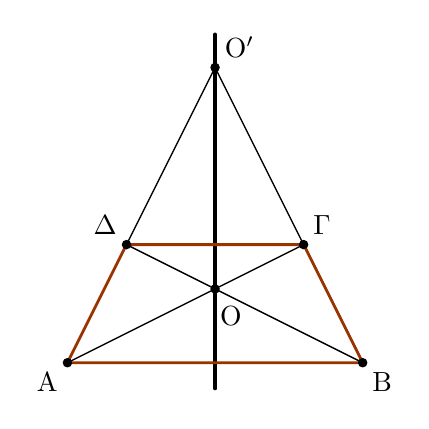
\begin{tikzpicture}[scale=.75]
\tkzSetUpLine[line width=1pt,color=black]
\tkzSetUpPoint[fill=black]

\tkzDefPoints{0/0/A,5/0/B,1/2/D,4/2/C}

\tkzDefPointBy[projection=onto C--D](A)\tkzGetPoint{A'}
\tkzDefPointBy[projection=onto A--B](D)\tkzGetPoint{D'}
\tkzInterLL(A,C)(B,D) \tkzGetPoint{O}
\tkzInterLL(A,D)(B,C) \tkzGetPoint{O'}

\tkzFillPolygon[fill=white](A,B,C,D)


\tkzDrawSegments[line width=0.5pt,color=black](A,O' B,O')

\tkzDrawSegments[line width=0.5pt,color=black](A,C B,D)
\tkzDrawSegments[line width=1.25pt,color=black,add=0.15 and 0.45](O',O)

\tkzDrawPolygon[color=ShapeClr](A,B,C,D)
\tkzDrawPoints[size=3](A,B,C,D,O,O')
\tkzLabelPoint[below left](A){$\rm A$}
\tkzLabelPoint[below right](B){$\rm B$}
\tkzLabelPoint[above right](C){$\rm \Gamma$}
\tkzLabelPoint[above left](D){$\rm \Delta$}
\tkzLabelPoint[xshift=0.2cm,yshift=-0.1cm](O){$\rm O$}
\tkzLabelPoint[above right](O'){$\rm O'$}

\end{tikzpicture}

\end{document}
